\renewcommand*{\arraystretch}{1.5}
\begin{tabularx}{15cm}{|p{2.1cm}@{\hskip 1ex}|@{\hskip 1ex}X|}
	\hline
	number      & 19                                                          \\ \hline
	title       & Stranger's interaction                                                           \\ \hline
	\multicolumn{2}{|c|}{ 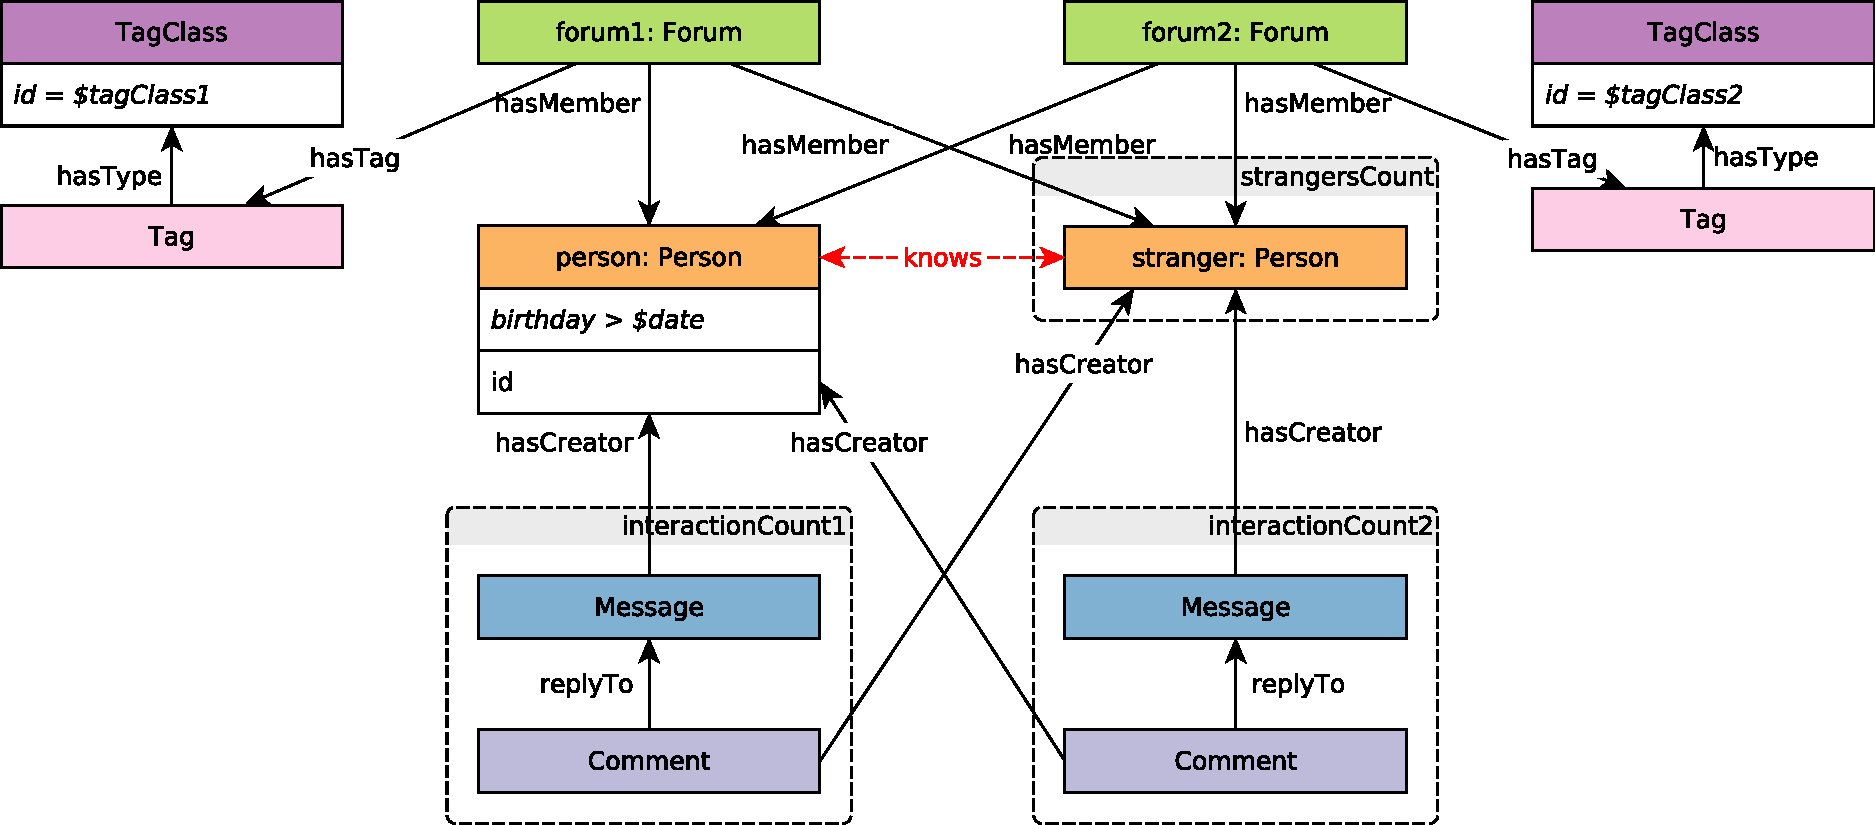
\includegraphics[scale=\patternscale,margin=0cm .2cm]{patterns/q19}} \\ \hline
	description & For all the Persons born after a certain date, find all the strangers
they interacted with, where strangers are Persons that do not Know each
other. There is no restriction on the date that strangers were born.

Consider only strangers that are members of Forums tagged with tagClass1
(direct children not transitive) AND members of Forums tagged with
tagClass2 (direct children not transitive). It does not matter if these
Tags are attached to the same Forum, or different Forums.

We define interaction as follows: a Person replies to a Message (Post or
Comment) by another Person.

For each Person, count the number of strangers they interacted
(directed) with and total number of times they interacted (directed)
with them.
 \\ \hline
	
	parameters  &
	\multicolumn{1}{>{\raggedright}X|}{
		\variable{date}{Date} \\
		\variable{tagClass1}{32bitInteger} \\
		\variable{tagClass2}{32bitInteger} 
		}\\ \hline
	result      &
	\multicolumn{1}{>{\raggedright}X|}{
		\variable{person.id}{64bitInteger}\\
		\variable{strangersCount}{32bitInteger}\\
		\variable{interactionCount}{32bitInteger}
		}\\ \hline
	sort        &
	\multicolumn{1}{>{\raggedright}X|}{
		\sortentry{interactionCount}{\desc}\\
		\sortentry{person.id}{\asc}
		}\\ \hline
	limit       & 100                                                           \\ \hline
	choke points        &
	\multicolumn{1}{>{\raggedright}X|}{
		\chokepoint{1.1}, 
		\chokepoint{1.4}, 
		\chokepoint{2.1}, 
		\chokepoint{2.3}, 
		\chokepoint{2.4}, 
		\chokepoint{3.3}, 
		\chokepoint{5.1}, 
		\chokepoint{7.3}, 
		\chokepoint{7.4}
		}\\ \hline
\end{tabularx}
\clearpage
